\documentclass[journal, letterpaper]{IEEEtran}
%\documentclass{scrartcl}

\usepackage[ngerman,english]{babel}
%\usepackage[latin1]{inputenc}
\usepackage[utf8]{inputenc}
\usepackage[T1]{fontenc}
\usepackage{amsmath}
\usepackage{amsthm}
\usepackage{amsfonts}
\usepackage{tikz}
\usepackage{verbatim}
\usepackage{subcaption}
\usepackage{algorithm}
\usepackage{algorithmic}
\usepackage[pdftex]{hyperref}

\renewcommand{\algorithmicrequire}{\textbf{Input:}}
\renewcommand{\algorithmiccomment}[1]{\ \ // #1} % C-like // Comments

\hyphenation{render}

% No clubs and widows allowed
\clubpenalty10000
\widowpenalty10000
\displaywidowpenalty=10000

\begin{document}

%\title{Simulating elastic spheres without external forces}
%\subtitle{Project 1 for class CS6491 Computer Graphics}
\title{Swirl \\
	{\large Project 2 for class CS6491 Computer Graphics}}
%\author{Sebastian Weiss}
\author{Sebastian Weiss, Kristian Eberhardson\\ \today}
%\date{\today}

\maketitle

\begin{tikzpicture}[remember picture,overlay]
   \node[anchor=north east,inner sep=0pt] at (current page.north east)
              {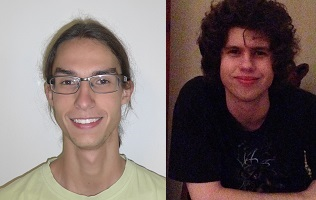
\includegraphics[scale=1.5]{pic}};
\end{tikzpicture}

\section{Objective}
We are provided with the starting and ending frame pair, call them $A_0$ and $A_1$.  We wish to create a continuous, affine and steady motion which interpolates $A_0$ and $A_1$.
 
\section{Input}
Assume $A_0$ and $A_1$ consist of a point P and a right hand coordinate system of orthogonal vectors I, J, and K, each of the same length.
\subsection{Terms} 
1. An \underline{affine} transformation in three dimensions can be expressed as a 4x4 matrix multiplied onto a point or a vector, is reversible, and can be expressed solely as a combination of rotation, translation, and scaling.
\newline
2. A \underline{continuous} transformation is one in which for any $\epsilon > 0$, there exists a $\delta > 0$ such that for any $0 <= t, u <= 1$, if $t - u < \delta$, then for any point x, $(A_u - A_t)x < \epsilon$.  Intuitively, this means I can draw the motion with a pen in a single stroke.
\newline
3. A \underline{steady} transformation preserves the angle between a pair of frames, and is independent of some time t. 

\section{Related interpolation schemes}

\subsection{Logarithmic spiral in 2D}
A series of pairwise adjacent frames converge to a fixed point F when the motion is repeated indefinitely.  This motion preserves the angle between each frame, which we denote $\alpha$.  This motion also uses the same scaling factor between each pair of adjacent frames, so we calculate $m = (A_1).length / (A_0).length$.  Because we estimate curves as lines consisting of finitely many points in Processing, we can recursively follow the motion to F, and the program will terminate in a finite amount of time; this is the approach Professor Rossignac uses in his project: "Patterns of Similar Frames and Interpolation".  The steps are to rotate the current frame A by $\alpha$ scale by m, and then have the function call itself with the new frame's parameters.  This coincidentally gives us all the in-between keyframes as well, since we are using them to find F. 

\subsection{Linear interpolation in 3D}
For all points in $A_0$, draw a straight line to its corresponding point in $A_1$.  Motion is simply moving the frame along these lines.  This is neither an elegant solution nor does it preserve the area of the frame.

\subsection{Projected log spiral + Translation}


\section{Proposed model}
We wish to create a swirling motion related to the logarithmic spiral but in 3D.  This means we need to calculate F, alpha, and m similarly to the 2D logarithmic spiral.

\subsection{3D rotation, first version}

\subsection{3D rotation, second version}


\subsection{Calculating $N$, $\alpha$ and $m$}
We calculate m just like we did in "Logarithmic Spiral in 2D", $m = (I_1).length / (I_0).length$ (since I, J, and K are of the same length, it does not matter which we use).  Then, $dI = I_1 - I_0$, $dJ = J_1 - J_0$, and $dK = K_1 - K_0$.  Then, we want to pick $N = dI\text{ x }dJ$ or $N = dI\text{ x }dK$ or $N = dJ\text{ x }dK$ depending on $\max{(|dI\text{ x }dJ|, |dI\text{ x  }dK|, |dJ\text{ x }dK|)}$.  
Let $pI0 = (I_0 \bullet N)N$, $pI1 = (I_1 \bullet N)N$, $pJ0 = (J_0 \bullet N)N$, $pJ1 = (J_1 \bullet N)N$, $pK0 = (K_0 \bullet N)N$, $pK1 = (K_1 \bullet N)N$.  Let $angle1$ denote the angle between $pI0$ and $pI1$, $angle2$ denote the angle between $pJ0$ and $pJ1$, and $angle3$ denote the angle between $pK0$ and $pK1$.  Then, $\alpha = \max{(angle1, angle2, angle3)}$. 

\subsection{Calculating $F$}

\subsection{Proof of steadiness}

\subsection{Dealing with special cases}
These are the cases in which there is either no fixed point or more than one around which our motion rotates steadily.

\subsubsection{No rotation}

\subsubsection{No rotation, no scaling}
(N = 0, have only translation)

\subsubsection{pure scaling}
For this case, we only need to calculate m.  Then, we can just scale the motion by m.

\section{Results}

\end{document}